\documentclass[ignorenonframetext,]{beamer}
\usepackage{amssymb,amsmath}
\usepackage{ifxetex,ifluatex}
\usepackage{fixltx2e} % provides \textsubscript
\ifxetex
  \usepackage{fontspec,xltxtra,xunicode}
  \defaultfontfeatures{Mapping=tex-text,Scale=MatchLowercase}
\else
  \ifluatex
    \usepackage{fontspec}
    \defaultfontfeatures{Mapping=tex-text,Scale=MatchLowercase}
  \else
    \usepackage[utf8]{inputenc}
  \fi
\fi
\usepackage{listings}
\lstset{basicstyle=\tiny}
\usepackage{graphicx}
% Para poner un fondo
\usebackgroundtemplate%
{%
    \Oldincludegraphics[width=\paperwidth,height=\paperheight]{../rsc/images/fondo-beamer.jpg}%
}

% Redefine \includegraphics so that, unless explicit options are
% given, the image width will not exceed the width of the page.
% Images get their normal width if they fit onto the page, but
% are scaled down if they would overflow the margins.
\makeatletter
\def\ScaleIfNeededW{%
  \ifdim\Gin@nat@width>\linewidth
    \linewidth
  \else
    \Gin@nat@width
  \fi
}
\def\ScaleIfNeededH{%
  \ifdim\Gin@nat@height>0.6\textheight
    0.6\textheight
  \else
    \Gin@nat@height
  \fi
}
\let\Oldincludegraphics\includegraphics
\renewcommand{\includegraphics}[2][]{\Oldincludegraphics[width=\ScaleIfNeededW, height=\ScaleIfNeededH,keepaspectratio]{#2}}

% Comment these out if you don't want a slide with just the
% part/section/subsection/subsubsection title:
\AtBeginPart{
  \let\insertpartnumber\relax
  \let\partname\relax
  \frame{\partpage}
}
\AtBeginSection{
  \let\insertsectionnumber\relax
  \let\sectionname\relax
  \frame{\sectionpage}
}
\AtBeginSubsection{
  \let\insertsubsectionnumber\relax
  \let\subsectionname\relax
  \frame{\subsectionpage}
}

\setlength{\parindent}{0pt}
\setlength{\parskip}{6pt plus 2pt minus 1pt}
\setlength{\emergencystretch}{3em}  % prevent overfull lines
\setcounter{secnumdepth}{0}


\begin{document}

\section{Más allá del core}\label{muxe1s-alluxe1-del-core}

\begin{frame}{Escalas}

\begin{itemize}
\item
  \textbf{Son funciones que nos facilitan el mapeo de datos a variables
  visuales}
\item
  En el API se llaman
  \href{https://github.com/mbostock/d3/wiki/API-Reference\#d3scale-scales}{scales}
\item
  Se utilizan sobre todo para relacionar el \textbf{dominio} de los
  datos con el \textbf{rango} de valores que tomarán al mapearlos a
  píxeles
\end{itemize}

\end{frame}

\begin{frame}[fragile]

\begin{lstlisting}
var w = 500;
var h = 2000;
var barMargin = 1;

var svg = d3.select(".chart")
    .append("svg")
    .attr("width", w)
    .attr("height", h);

d3.csv("cars.csv", function (cars) {
       render(cars);
       });
           
var render = function(datos) {
    
    var weights = datos.map(function(d){
                return parseInt(d['weight (lb)']);});

    /**
     * Adaptado al alto del SVG
     * 
     * El redondeo evita problemas de aliasing
     */
    var barWidth = Math.floor( (h / weights.length) - barMargin );

    svg.selectAll('.bar')
    .data(weights)
      .enter()
    .append('rect')
    .attr('class', 'bar')
    .attr('y', function(d,i) {return i*(barWidth+barMargin);})
    .attr('width', function(d){return d * 0.05;})
    .attr('height', barWidth);
};
\end{lstlisting}

\end{frame}

\begin{frame}{Ejercicio 11}

\begin{itemize}
\itemsep1pt\parskip0pt\parsep0pt
\item
  Sobre el código del Ejercicio 10:

  \begin{itemize}
  \itemsep1pt\parskip0pt\parsep0pt
  \item
    Ajustar los tamaños, horizontales y verticales, de las barras
    utilizando una
    \href{https://github.com/mbostock/d3/wiki/Quantitative-Scales\#linear}{escala
    lineal}
  \end{itemize}
\end{itemize}

\end{frame}

\begin{frame}{Ejercicio 12}

\begin{itemize}
\itemsep1pt\parskip0pt\parsep0pt
\item
  Orienta el diagrama de barras para que las barras queden verticales
\end{itemize}

\begin{figure}[htbp]
\centering
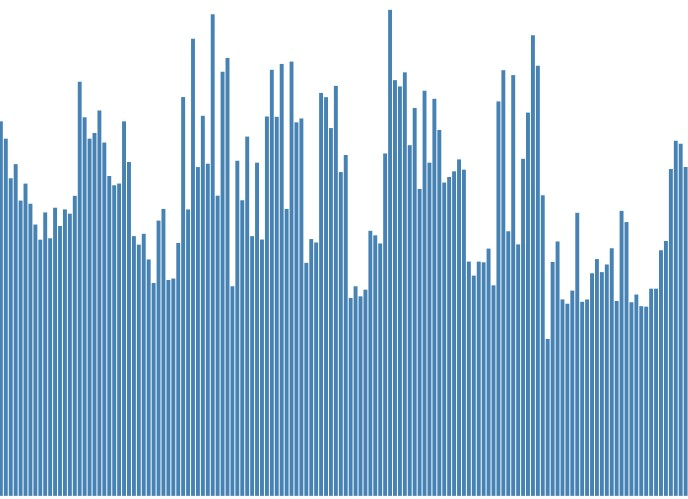
\includegraphics{../rsc/images/ej12.jpg}
\end{figure}

\end{frame}

\begin{frame}{Layouts}

\begin{itemize}
\item
  Los \href{https://github.com/mbostock/d3/wiki/Layouts}{layout} no son
  más que una transformación de datos, \textbf{no dibujan nada}.
\item
  Ayudan a calcular los valores de las variables gráficas que van a
  representar los datos
\end{itemize}

\end{frame}

\begin{frame}[fragile]{Tooltips}

\begin{itemize}
\item
  Son pequeños textos que nos dan información de detalle sobre un
  elemento.
\item
  Se muestran cuando nos posamos sobre algún elemento.
\item
  La manera más fácil es utilizar el elemento \textbf{title} de SVG

\begin{lstlisting}
<circle><title>Este el mensaje del tooltip</title></circle>
\end{lstlisting}
\end{itemize}

\end{frame}

\begin{frame}{Ejercicio 13}

\begin{figure}[htbp]
\centering
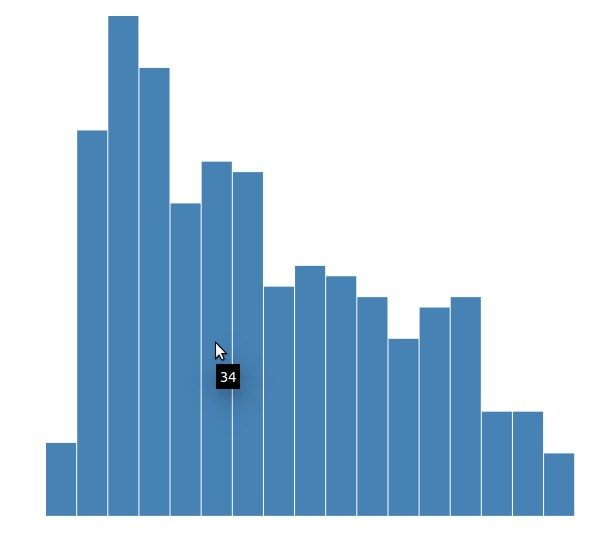
\includegraphics{../rsc/images/ej13.jpg}
\end{figure}

\end{frame}

\begin{frame}

\begin{itemize}
\item
  Utiliza el \textbf{layout
  \href{https://github.com/mbostock/d3/wiki/Histogram-Layout}{histogram}}
  para crear un histograma de pesos con 20 barras
\item
  Para definir los 20 bins utiliza el método \textbf{ticks} de tu escala
  horizontal
\item
  Añade un tooltip en cada barra con su valor (el peso del coche)
\end{itemize}

\end{frame}

\begin{frame}[fragile]{Ejes}

\begin{itemize}
\item
  Son funciones del módulo \textbf{d3.svg} que \textbf{pintan} los ejes
\item
  En el API se llaman
  \href{https://github.com/mbostock/d3/wiki/SVG-Axes}{axes}
\item
  Se utilizan siempre en conjunción con las \textbf{escalas}
\item
  Desde la selección del elemento padre ejecutamos nuestro eje ya
  configurado.

\begin{lstlisting}
var yAxis = d3.svg.axis() // Es un clousure
    .scale(y)
    .orient("left");

svg.call(yAxis);
\end{lstlisting}
\end{itemize}

\end{frame}

\begin{frame}[fragile]

\begin{itemize}
\itemsep1pt\parskip0pt\parsep0pt
\item
  Es necesario darles un estilo con CSS:
\end{itemize}

\begin{lstlisting}
.axis text {
  font: 10px sans-serif;
}

.axis path,
.axis line {
  fill: none;
  stroke: #000;
  shape-rendering: crispEdges;
}
\end{lstlisting}

\end{frame}

\begin{frame}{Groups en SVG}

\begin{itemize}
\item
  El elemento \textbf{g} es sólo un contenedor
\item
  Se puede utilizar para hacer \textbf{capas} (SVG se renderiza con el
  algoritmo del pintor)
\item
  Muy utilizado para aplicar
  \href{http://tutorials.jenkov.com/svg/svg-transformation.html}{transformaciones}
  a muchos elementos
\end{itemize}

\end{frame}

\begin{frame}[fragile]{Márgenes}

Existe una convención para poner márgenes a la gráfica. Útil para poner
los ejes en ellos.

\begin{lstlisting}
var margin = {top: 10, right: 30, bottom: 30, left: 30};
var width = 960 - margin.left - margin.right;
var height = 500 - margin.top - margin.bottom;

var svg = d3.select("body").append("svg")
    .attr("width", width + margin.left + margin.right)
    .attr("height", height + margin.top + margin.bottom)
  .append("g")
    .attr("transform", "translate(" + margin.left + "," + margin.top + ")");
\end{lstlisting}

\end{frame}

\begin{frame}{Ejercicio 14}

\begin{figure}[htbp]
\centering
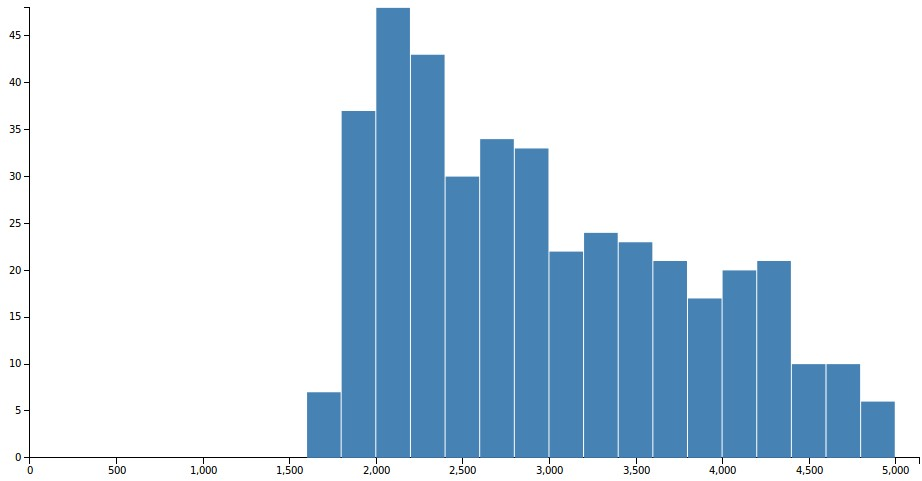
\includegraphics{../rsc/images/ej14.jpg}
\end{figure}

\end{frame}

\begin{frame}

\begin{itemize}
\itemsep1pt\parskip0pt\parsep0pt
\item
  Añade dos ejes con
  \textbf{\href{https://github.com/mbostock/d3/wiki/SVG-Axes}{svg.axis}},
  a la coordenada X y a la Y
\item
  Utiliza la convención de márgenes para situar los ejes fuera de la
  gráfica
\item
  Mejora la legibilidad de los ejes con CSS
\end{itemize}

\end{frame}

\begin{frame}{Ejercicio 15}

\begin{figure}[htbp]
\centering
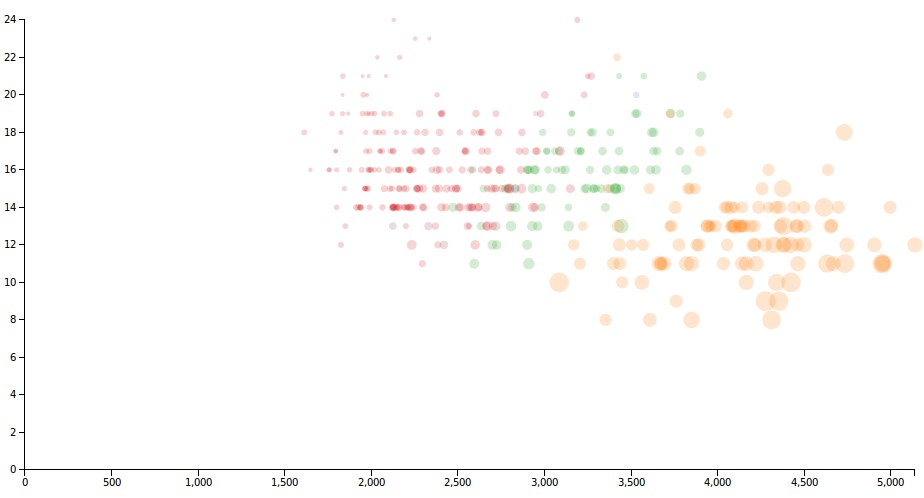
\includegraphics{../rsc/images/ej15.jpg}
\end{figure}

\end{frame}

\begin{frame}

\begin{itemize}
\item
  Scatter plot de ``weight (lb)'' (eje X) y ``0-60 mph (s)'' (eje Y)
\item
  Círculos con radio mapeando el ``power (hp)'' (escala lineal)
\item
  Color mapeando el número de cilindros ``cylinders''
  (\href{https://github.com/mbostock/d3/wiki/Ordinal-Scales\#category10}{category10})
\item
  Tooltip muestra el nombre ``name''
\item
  Ejes X e Y.
\item
  Utiliza la convención de márgenes para situar los ejes fuera de la
  gráfica
\end{itemize}

\end{frame}

\begin{frame}[fragile]{Interacción}

\begin{itemize}
\item
  Cualquier elemento del DOM puede ser interactivo
\item
  Con d3, cualquier selección tiene un método \textbf{on} para capturar
  eventos y tratarlos con callbacks

\begin{lstlisting}
d3.selectAll("rect").on("click", function(d){});
\end{lstlisting}
\item
  \href{http://www.w3.org/TR/SVG11/interact.html}{Lista} de eventos
  comunes en SVG: click, mousedown, mouseup, mouseover, mouseout
\item
  Funciones útiles: \textbf{d3.mouse} y \textbf{d3.event}
\end{itemize}

\end{frame}

\begin{frame}[fragile]{Ejercicio 16}

\begin{itemize}
\item
  Utiliza la metaclase ``:hover'' para dibujar un stroke

\begin{lstlisting}
p:hover { color:red; }  /* Código CSS */
\end{lstlisting}
\item
  Cuando se pincha ( on(``click'', callback) ) en un coche se muestra un
  mensaje con el mandato ``alert'' que tiene el número de cilindros del
  coche

\begin{lstlisting}
// Prueba en la consola de javascript
alert("hola mundo");
\end{lstlisting}
\item
  Cuando se pasa por encima con el ratón, peso y velocidad se muestran
  en un ``p'' arriba de la gráfica

  \begin{itemize}
  \itemsep1pt\parskip0pt\parsep0pt
  \item
    Añade el p en el html con una clase para identificarlo
  \item
    El evento a capturar es \textbf{mouseover}
  \item
    Modifica el \textbf{text} del \textbf{p} desde d3
  \end{itemize}
\end{itemize}

\end{frame}

\end{document}
